Module CPU Top là bước tích hợp mức cao nhất (Top-level Instantiation), 
nơi toàn bộ các khối chức năng con và khối điều khiển được liên kết với nhau
 để tạo thành một vi xử lý RISC 8-pha.
\begin{figure}[H]
    \centering
    % Nhớ đổi tên file ảnh dưới đây cho khớp với tên file bạn lưu trong máy nhé
    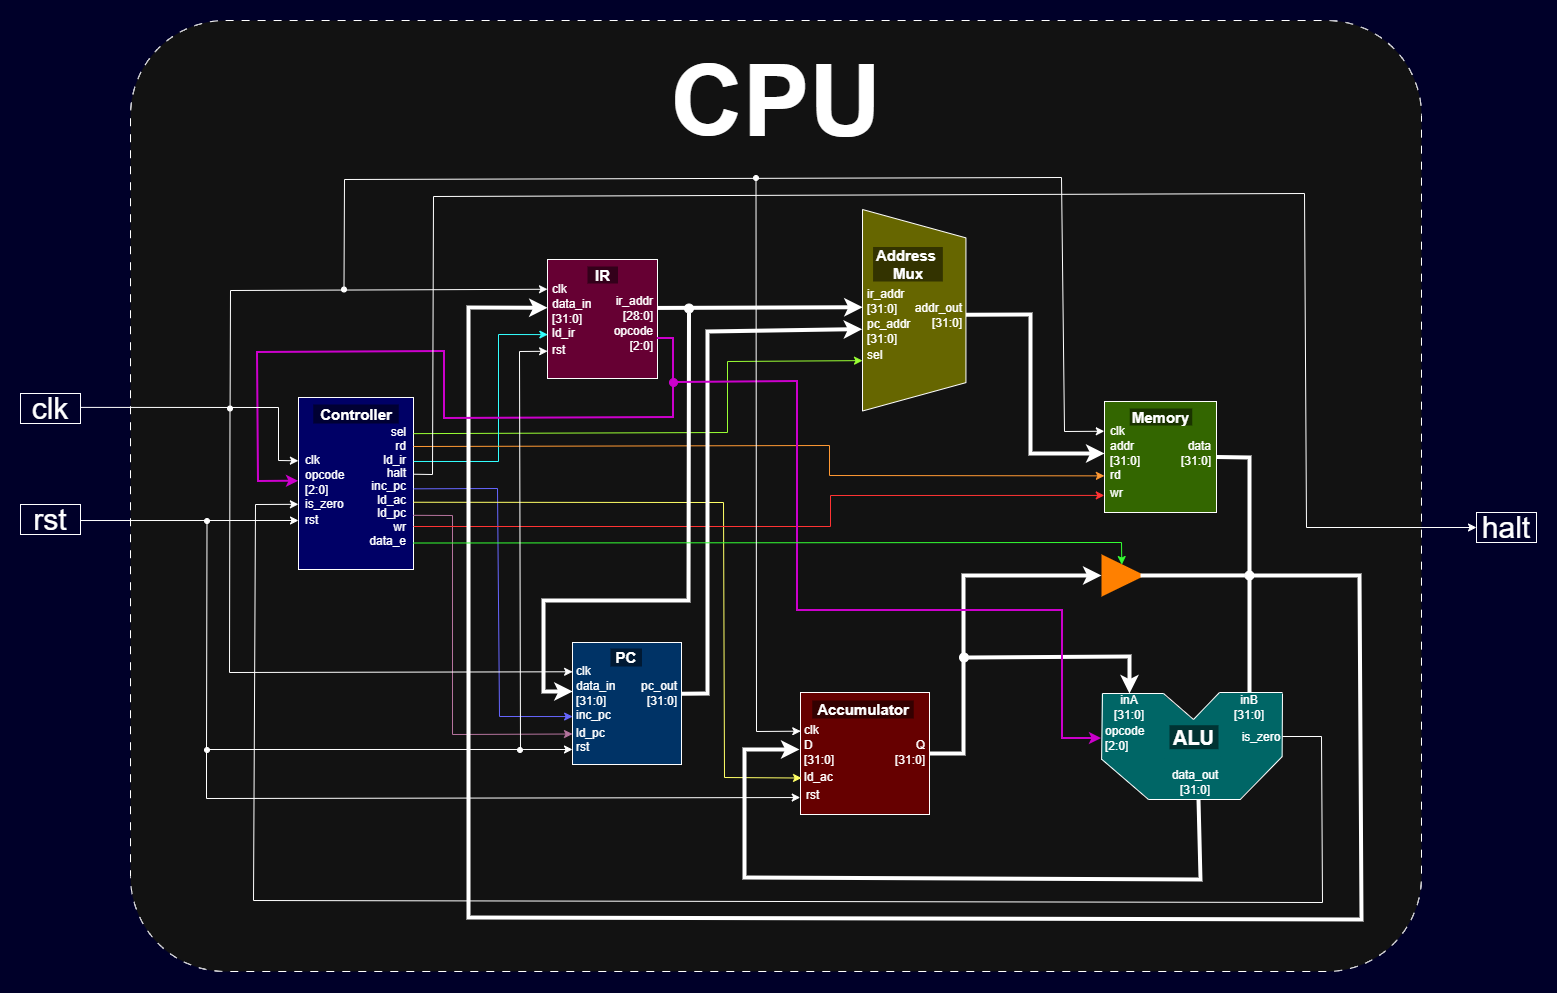
\includegraphics[width=\textwidth]{CPU.png} 
    \caption{Kiến trúc tổng thể và luồng dữ liệu của CPU}
    \label{fig:cpu_top_diagram}
\end{figure}

\textbf{Phân tích cấu trúc kết nối hệ thống:}

Nhìn vào Sơ đồ \ref{fig:cpu_top_diagram}, 
có thể thấy kiến trúc tổng thể của CPU được chia làm hai hệ thống 
mạng lưới dây dẫn biệt lập, hoạt động đan xen nhau:

\begin{itemize}
    \item \textbf{Đường dẫn dữ liệu (Datapath - Các đường bus 32-bit nét đậm):} 
    Đảm nhiệm việc vận chuyển mã lệnh, địa chỉ và toán hạng giữa các khối chức năng.
    \begin{itemize}
        \item \textbf{Định tuyến Địa chỉ (Address Routing):} Địa chỉ truy cập bộ nhớ được lựa chọn qua khối Address Mux. Trong pha Fetch, địa chỉ được cấp từ \texttt{PC}. Trong pha Execute, địa chỉ được cấp từ trường \texttt{ir\_addr} của \texttt{IR}.
        \item \textbf{Định tuyến Lệnh nhảy (Jump Routing):} Một nhánh của bus \texttt{ir\_addr} được nối trực tiếp vào ngõ vào \texttt{data\_in} của \texttt{PC}. Đây là đường dẫn dữ liệu phần cứng cốt lõi để thực thi lệnh rẽ nhánh không điều kiện (\texttt{JMP}).
        \item \textbf{Vòng lặp tính toán (ALU Execution Loop):} Mọi phép toán đều lấy thanh ghi \texttt{Accumulator} làm trung tâm. Toán hạng thứ nhất (\texttt{inA}) luôn được cấp từ ngõ ra của Accumulator, trong khi toán hạng thứ hai (\texttt{inB}) được lấy trực tiếp từ bus dữ liệu của \texttt{Memory}.
        \item \textbf{Lưu trữ dữ liệu (Store Path):} Khối đệm 3 trạng thái (Tristate Buffer) được đặt giữa Accumulator và bus bộ nhớ. Khi cần thực thi lệnh \texttt{STO}, cổng này mở ra, cho phép dữ liệu từ Accumulator chảy ngược lên bus chung để ghi vào bộ nhớ.
    \end{itemize}
    
    \item \textbf{Đường dẫn điều khiển (Control Path - Các đường tín hiệu 1-bit nét thanh):} 
    \begin{itemize}
        \item Khối \texttt{Controller} đóng vai trò là nhạc trưởng. Nó liên tục lắng nghe mã lệnh \texttt{opcode} từ \texttt{IR} và cờ \texttt{is\_zero} phản hồi từ \texttt{ALU}.
        \item Dựa trên Máy trạng thái 8 pha, \texttt{Controller} sẽ kích hoạt các tín hiệu điều khiển (như \texttt{sel, rd, wr, inc\_pc, ld\_ac...}) tới chân Enable của từng khối logic tại các nhịp clock tương ứng. Việc phân chia tín hiệu độc lập đảm bảo hệ thống vận hành tuần tự, không bao giờ xảy ra tình trạng đụng độ dữ liệu (Data Hazard) trên bus hệ thống.
    \end{itemize}
\end{itemize}